\documentclass{standalone}
\usepackage{pgf}
\usepackage{amsmath}
\usepackage{tikz}
\usetikzlibrary{shapes,arrows}
\usetikzlibrary{positioning}
\begin{document}
   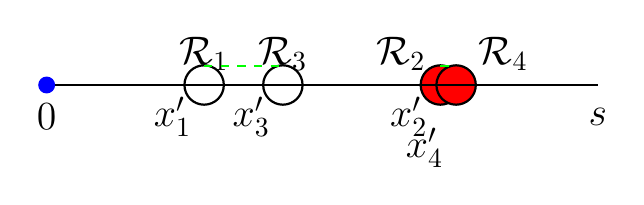
\begin{tikzpicture}
\coordinate  (a) at (0,0);
\coordinate  (b) at (1,0);
\coordinate  (c) at (3.,0);
\coordinate  (d) at (3.2,0) ;

\draw[thick] (a) circle (0.25cm);
 \node[draw=none,align=left] at (0,0.4) {\Large $\mathcal{R}_1$};
\node[draw=none,align=left] at (-0.4,-0.4) {\Large $x_1'$} ;

\draw[thick] (b) circle (0.25cm);
 \node[draw=none,align=left] at (1,0.4) {\Large $\mathcal{R}_3$};
\node[draw=none,align=left] at (0.6,-0.4) {\Large $x_3'$} ;

\draw[dashed,thick,green] (0,0.24) -- (1,0.24);

\draw[thick,fill=red] (c) circle (0.25cm);
\node[draw=none,align=left] at (2.5,0.4) {\Large $\mathcal{R}_2$};
\node[draw=none,align=left] at (2.6,-0.4) {\Large $x_2'$} ;

\draw[thick,fill=red] (d) circle (0.25cm);
\node[draw=none,align=left] at (3.8,0.4) {\Large $\mathcal{R}_4$};
\node[draw=none,align=left] at (2.8,-0.8) {\Large $x_4'$} ;



\draw[thick] (-2,0) -- (+5,0);


\draw[blue,fill=blue] (-2,0) circle (.1cm); 
 \node[draw=none,align=left] at (-2.0,-0.4) {\Large $0$};
 \node[draw=none,align=left] at (5,-0.4) {\Large $s$};

\draw[dashed,thick,green] (3,0.24) -- (3.2,0.24);


\end{tikzpicture}
\end{document}

